Terminata la fase esplorativa, i concept selezionati sono stati trasformati in prototipi digitali a media fedeltà (wireframe).
Al fine di tradurre gli sketch manuali in layout interattivi e navigabili, per la modellazione delle interfacce è stato adottato Figma, strumento di riferimento per la progettazione UI/UX.
Lavorare con questo livello di fedeltà intermedio ha consentito di definire con precisione l'architettura dell'informazione, i flussi di navigazione e la disposizione spaziale dei componenti.
Infine, la scelta di mantenere le schermate in scala di grigi è nata dalla necessità di concentrare l'analisi sui soli aspetti strutturali, ergonomici e funzionali.
Di conseguenza, le variabili cromatiche e stilistiche sono state escluse temporaneamente, pur riconoscendo la loro importanza in un'applicazione dedicata al benessere mentale.

In questo passaggio le interfacce definite in fase di sketch sono state ricostruite in ambiente digitale e, laddove il confronto teorico non aveva individuato un'opzione prevalente, si è proceduto a modellare entrambe le alternative.
È il caso della pagina del diario e della vista di dettaglio delle richieste di aiuto (\textbf{REQ-07}), per le quali sono state realizzate due versioni destinate al confronto empirico con gli utenti.
Il maggiore grado di dettaglio ha inoltre permesso di verificare la tenuta dei layout e la gerarchia visiva sulle dimensioni reali di uno schermo mobile, facendo emergere alcune correzioni rispetto ai prototipi disegnati a mano che vengono discusse nelle sezioni corrispondenti.

\section{Struttura di navigazione e layout}
\label{sec:wireframe-struttura}

Il passaggio alla media fedeltà ha consentito di verificare e dimensionare con precisione il sistema di navigazione già ipotizzato in fase esplorativa, misurandone l'ingombro effettivo sulla risoluzione di uno schermo mobile di riferimento.
Il lavoro non ha modificato la struttura definita con gli sketch, ma ne ha stabilito le proporzioni, le distanze e le aree sensibili al tocco.

La navigazione primaria resta affidata a una barra inferiore persistente, che separa le tre aree principali dell'applicazione, ovvero la schermata di supporto emotivo, il diario personale e il profilo.
La scelta di una navigazione sempre visibile anziché di un menu richiamabile con un gesto discende dalle evidenze presentate nelle linee guida, secondo le quali qualsiasi metodo di navigazione nascosto risulta meno individuabile e conduce a un utilizzo ridotto delle funzioni che nasconde.
Gli stessi confronti indicano nella barra inferiore il pattern che consente i tempi di navigazione più brevi rispetto al menu laterale e alla barra superiore a schede, e in un'applicazione destinata a essere aperta durante una crisi ogni passaggio risparmiato ha un peso concreto (\textbf{REQ-04}).
La scheda attiva è stata inoltre evidenziata rispetto alle altre, in modo che l'utente riconosca sempre il proprio punto di posizione all'interno dell'applicazione.

La fascia superiore adotta un blocco pieno che occupa l'intera larghezza e ospita il titolo della sezione corrente accompagnato da una breve riga esplicativa.
Il contrasto fra questa fascia e il fondo chiaro del corpo della pagina fornisce a ogni schermata una cornice riconoscibile e costante, mentre l'area compresa fra le due estremità resta interamente disponibile ai contenuti, organizzati in card che scorrono verticalmente.
La distinzione fra la navigazione collocata in basso e le informazioni di contesto collocate in alto mantiene una gerarchia visiva pulita e previene il sovraccarico cognitivo (\textbf{REQ-01}).

Nelle schermate che chiedono all'utente di procedere, ovvero quelle del flusso di aiuto e le viste di dettaglio del diario, il comando principale è stato collocato nella porzione inferiore dell'area di contenuto, dove le linee guida individuano la zona di naturale estensione del pollice nell'uso a una mano.
Le dimensioni degli elementi interattivi sono state verificate rispetto alle misure minime raccomandate per i target tattili, così che restino raggiungibili anche da chi li preme con la mano tremante.

\section{Schermata di accesso: login e creazione account}
\label{sec:wireframe-accesso}

La progettazione dell'area di accesso si fonda sulla massima rassicurazione e sulla riduzione dell'attrito iniziale.
Nella porzione superiore lo spazio è dominato dal logo dell'applicazione inserito in un blocco scuro che definisce l'identità visiva del brand.
Il modulo centrale di autenticazione accoglie l'utente con un messaggio di benvenuto e istruzioni chiare, racchiudendo in un layout verticale pulito i campi per l'inserimento di email e password.
Quest'ultimo campo integra un'icona dedicata alla visibilità del testo, offrendo un riscontro immediato e prevenendo errori di digitazione.

Accanto al pulsante principale di accesso è stata inserita un'opzione strategica fondamentale per un'applicazione focalizzata sul benessere mentale: il comando per continuare come ospite.
Questa scelta di design permette di bypassare la registrazione immediata riducendo drasticamente l'ansia da prestazione o la frustrazione di un utente che necessita di supporto rapido.
Al di sotto del box principale trovano spazio il link per il recupero della password e un'icona con un messaggio esplicito sulla privacy e sulla protezione delle riflessioni personali.
Infine, la barra inferiore ospita il rinvio alla schermata di registrazione, completando un'architettura che bilancia sicurezza, flessibilità e immediatezza d'uso.

\begin{figure}[htbp]
    \centering
    
\includegraphics[height=8cm]{imgs/wireframes/login.png}
    \caption{Wireframe dell'accesso}
    \label{fig:wireframe-login}
\end{figure}

La schermata di creazione del profilo riprende integralmente l'impostazione di quella di accesso, così che il passaggio dall'una all'altra non richieda alcun riorientamento.
La fascia superiore ospita il titolo dell'operazione accompagnato da una riga che ne dichiara la natura locale, mentre il corpo raccoglie in un unico modulo verticale i campi necessari all'identificazione del profilo, ovvero nome, cognome, indirizzo di posta elettronica e password con la relativa conferma.
I campi sono disposti in sequenza verticale e ciascuno è preceduto dalla propria etichetta, mentre la conferma della password segue immediatamente il campo a cui si riferisce, così che un errore di digitazione emerga durante l'inserimento anziché al momento dell'invio.

L'intestazione mantiene un comando di ritorno alla schermata precedente, coerentemente con il principio di reversibilità che governa l'intera applicazione (\textbf{REQ-03}), e nessun passaggio di configurazione viene interposto fra la creazione del profilo e l'accesso alle funzioni (\textbf{REQ-04}).
Al di sotto del pulsante di conferma trova infine posto un messaggio esplicito sul trattamento dei dati, collocato deliberatamente nel punto in cui all'utente viene chiesto di consegnarli.
La rassicurazione sulla conservazione esclusivamente locale delle informazioni (\textbf{REQ-05}) compare quindi nel momento esatto in cui diventa pertinente, anziché essere relegata a un documento che nessuno leggerebbe.

\begin{figure}[htbp]
    \centering
    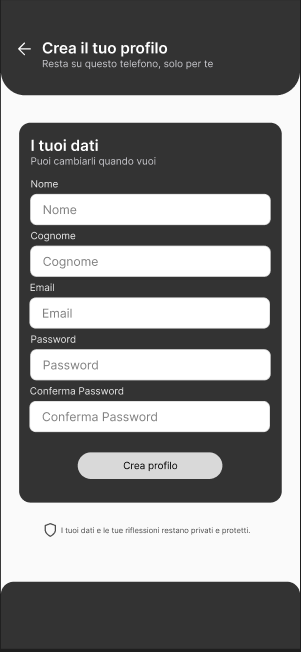
\includegraphics[height=8cm]{imgs/wireframes/signin.png}
    \caption{Wireframe della creazione del profilo}
    \label{fig:wireframe-registrazione}
\end{figure}

\section{Schermata principale: dashboard di supporto emotivo}
\label{sec:wireframe-principale}

Lo sviluppo del wireframe per la schermata principale ha permesso di tradurre in veste grafica le riflessioni emerse in fase esplorativa.
Nello specifico, il pulsante di emergenza è stato leggermente ridimensionato e riposizionato rispetto al centro assoluto per evitare di generare ulteriore allarmismo durante un attacco.
Inoltre, si è deciso di non renderlo l'unico elemento della homepage, pur mantenendo l'interfaccia semplice e con un carico informativo ridotto.
L'elemento mantiene comunque una priorità gerarchica chiara e non passa in secondo piano.
Lavorare a questo livello di dettaglio ha consentito di bilanciare accuratamente i pesi visivi e la distribuzione delle informazioni sul dispositivo.

\begin{figure}[htbp]
    \centering
    
\includegraphics[height=8cm]{imgs/wireframes/homepage.png}
    \caption{Wireframe della schermata principale}
    \label{fig:wireframe-homepage}
\end{figure}

L'architettura modulare della schermata è stata studiata per bilanciare l'immediata leggibilità generale con la rapida individuazione delle funzioni di supporto.
Il pulsante di emergenza (\enquote{Ho bisogno di aiuto}) sfrutta il contrasto visivo e l'isolamento spaziale per emergere in modo inequivocabile.
Tuttavia, non essendo l'elemento di maggiori dimensioni in assoluto, garantisce visibilità senza generare un senso di allarme o urgenza ansiogena.
Parallelamente, la sezione delle attività consigliate è concepita come una scorciatoia ad accesso rapido, che permette di avviare un esercizio di stabilizzazione in autonomia senza attivare una sessione di soccorso vera e propria, mentre la card dei progressi restituisce l'andamento delle richieste nel tempo.

Coerentemente con la natura di un prototipo a media fedeltà, si è optato per l'impiego di forme geometriche e placeholder in scala di grigi.
Questa impostazione permette di abbattere il carico cognitivo derivante da colori o immagini dettagliate, focalizzando l'analisi esclusivamente sull'architettura della Home, sull'allineamento delle card e sulla fluidità di fruizione del supporto psicologico.

\section{Flusso di aiuto: transizione e attività di supporto}
\label{sec:wireframe-flusso}

Per guidare l'utente verso le attività di supporto è stata progettata una schermata di transizione in linea con gli sketch esplorativi.
Questa interfaccia, che l'utente può decidere di saltare con un semplice tocco, ha lo scopo di confortare la persona, cercando di metterla a proprio agio.
L'obiettivo è offrire un primo momento di rassicurazione, pur essendo consapevoli dell'estrema difficoltà emotiva che caratterizza un attacco di panico.

\begin{figure}[htbp]
    \centering
    
\includegraphics[height=8cm]{imgs/wireframes/transizione.png}
    \caption{Wireframe della schermata di transizione}
    \label{fig:wireframe-transizione}
\end{figure}

Le tre attività di supporto vengono ora esaminate a livello di media fedeltà, ciascuna nella propria sezione.

Si segnala che i wireframe di queste schermate conservano la barra di navigazione inferiore per uniformità con il resto dell'applicazione, benché gli sketch esplorativi l'avessero omessa.
La contraddizione fra le due soluzioni è stata deliberatamente lasciata aperta e portata alla valutazione con gli utenti, poiché soltanto osservando qualcuno interrompere una sessione si poteva stabilire se quelle tre schede costituissero una comodità oppure una via d'uscita involontaria, capace di far perdere i progressi dell'esercizio in un momento di particolare fragilità.

\subsection{Attività 1: respirazione guidata}
\label{subsec:wireframe-respirazione}

L'interfaccia dedicata alla respirazione centralizza il focus visivo dell'utente tramite un indicatore circolare di grandi dimensioni posizionato al centro del viewport.
Questa scelta geometrica asseconda il ritmo della tecnica, fornendo un feedback visivo continuo che accompagna le delicate fasi di inspirazione ed espirazione.
Per garantire il pieno controllo dell'esperienza, è stato inserito un comando inferiore che permette di eludere le pause di mantenimento.
L'assenza di elementi periferici superflui minimizza le distrazioni, convogliando tutta l'attenzione sull'esercizio respiratorio e sul ripristino della calma.

\begin{figure}[htbp]
    \centering
    
\includegraphics[height=8cm]{imgs/wireframes/task-1.png}
    \caption{Wireframe della respirazione guidata}
    \label{fig:wireframe-task1}
\end{figure}

\subsection{Attività 2: distrazione cognitiva}
\label{subsec:wireframe-distrazione}

Per l'esercizio di riorientamento attentivo, il layout abbandona la tradizionale rigidità strutturale a favore di una disposizione sparsa e apparentemente casuale degli elementi interattivi.
La schermata invita l'utente a interagire con diverse sagome a forma di stella distribuite sull'intero spazio di lavoro.
Questa microinterazione tattile funge da ancoraggio nel momento presente, interrompendo efficacemente il sovraccarico ansioso.
Il riempimento delle forme al tocco fornisce un rinforzo visivo immediato, premiando l'azione e incentivando la prosecuzione del compito senza generare alcun tipo di stress aggiuntivo.

\begin{figure}[htbp]
    \centering
    
\includegraphics[height=8cm]{imgs/wireframes/task-2.png}
    \caption{Wireframe dell'attività delle stelle}
    \label{fig:wireframe-task2}
\end{figure}

\subsection{Attività 3: grounding 5-4-3-2-1}
\label{subsec:wireframe-grounding}

La tecnica di grounding spaziale sfrutta un pattern di navigazione verticale a step progressivi, riprendendo la logica visiva di una timeline.
Questa architettura frammenta il compito cognitivo in porzioni facilmente assimilabili, riducendo drasticamente lo sforzo di lettura per un utente in stato di agitazione.
La forte gerarchia tipografica separa in modo netto i numeri chiave dalle istruzioni operative, guidando lo sguardo in modo ordinato.
Lo scorrimento dell'interfaccia svela gradualmente i passaggi successivi, accompagnando dolcemente la persona verso il completamento della procedura sensoriale.

\begin{figure}[htbp]
    \centering
    
\includegraphics[height=8cm]{imgs/wireframes/task-3.png}
    \caption{Wireframe del grounding 5-4-3-2-1}
    \label{fig:wireframe-task3}
\end{figure}

\subsection{Attività conclusiva: questionario di feedback}
\label{subsec:wireframe-questionario}

La fase finale del processo di stabilizzazione prevede la compilazione di un breve questionario del tutto opzionale.
L'inserimento di questo passaggio permette di tracciare l'evoluzione emotiva dell'utente, rispettando pienamente i suoi tempi di recupero.
Occorre inoltre evidenziare una scelta progettuale trasversale a tutto il flusso, ovvero che l'interruzione volontaria del percorso è consentita in ogni momento.
Progettare interfacce prive di vie di fuga rischia infatti di amplificare la sensazione di panico.
L'integrazione di un comando di uscita sempre disponibile spezza le dinamiche mentali che favoriscono l'ansia, conferendo all'utente una totale autonomia decisionale.

\begin{figure}[htbp]
    \centering
    
\includegraphics[height=8cm]{imgs/wireframes/questionario.png}
    \caption{Wireframe del questionario di chiusura}
    \label{fig:wireframe-questionario}
\end{figure}

Il passaggio alla media fedeltà ha inoltre sciolto due questioni che gli sketch avevano lasciato aperte.
Il fattore scatenante, per il quale l'esplorazione si era limitata a registrare la necessità di un modo per descriverlo, viene ora indicato premendo una fra le etichette già presenti sullo schermo, alle quali se ne affianca una generica che consente di rispondere anche quando la causa non rientra fra quelle previste, senza costringere l'utente a formulare una descrizione.
Fra le domande di chiusura compare poi l'interrogativo sullo stato dell'utente in quel momento, al quale è stata associata la possibilità di avviare immediatamente un'altra sessione.
La scelta nasce dal riconoscimento che il percorso di soccorso può non risultare sufficiente al primo tentativo, e che in tal caso obbligare la persona a tornare alla schermata principale e a premere nuovamente il pulsante di aiuto costituirebbe un attrito inutile in un momento di fragilità.

\section{Schermata Diario: tracking delle crisi e riflessione personale}
\label{sec:wireframe-diario}

Per il tracking delle crisi, per il monitoraggio dello stato emotivo e per l'inserimento di una riflessione a freddo, pensata per i momenti in cui l'utente si trova in una condizione di calma, sono state modellate entrambe le opzioni ideate nella fase precedente.

L'obiettivo è stato quello di realizzare due interfacce interattive per la pagina del diario e per la vista estesa delle richieste d'aiuto da mettere a confronto.
Questo approccio ha permesso di valutare empiricamente il miglior punto di equilibrio tra rapidità operativa e completezza della raccolta dati.

Osservando la prima proposta per la sezione principale del diario si nota l'adozione di un layout pressoché tabulare per la card delle richieste di aiuto.
Questa struttura includeva anche il fattore scatenante dell'attacco, ma risultava complessa da scansionare a colpo d'occhio, rendendo difficile percepire immediatamente l'intensità della crisi.

\begin{figure}[htbp]
    \centering
    
\includegraphics[height=8cm]{imgs/wireframes/diario.png}
    \caption{Prima proposta per il diario, con la card delle richieste in forma di tabella}
    \label{fig:wireframe-diario-a}
\end{figure}

Nella seconda proposta la card conserva le tre informazioni essenziali di ciascun episodio, ovvero il numero progressivo, l'orario in cui la richiesta è stata avviata e l'intensità dichiarata.
Quest'ultima non è più esposta come semplice frazione numerica ma affidata a un indicatore che affianca al valore un riempimento proporzionale, leggibile senza doverlo interpretare.
Il fattore scatenante, presente nella versione precedente, è stato spostato nella vista di dettaglio, dove lo spazio disponibile consente di riportarlo per esteso.
Sotto le righe visibili resta un accenno grafico alla presenza di ulteriori registrazioni, che segnala la continuazione dell'elenco senza occupare altezza e invita ad aprire la vista estesa (\textbf{REQ-07}).

\begin{figure}[htbp]
    \centering
    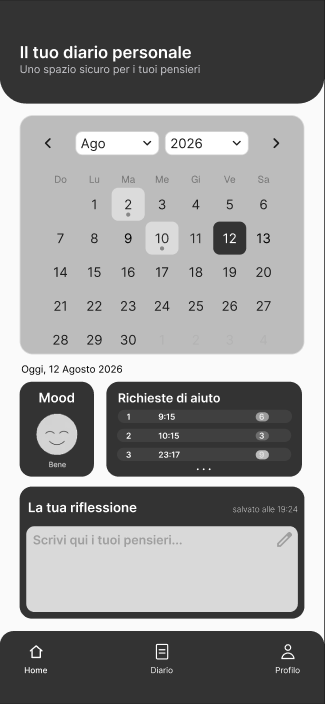
\includegraphics[height=8cm]{imgs/wireframes/diario-final.png}
    \caption{Seconda proposta per il diario, con l'intensità affidata a un indicatore proporzionale}
    \label{fig:wireframe-diario-b}
\end{figure}

Pur presentando un layout pressoché identico alla versione precedente, questa proposta interviene su un solo dettaglio visivo, ovvero il modo in cui viene comunicata l'intensità, ed è proprio per questo che è stata portata al confronto con gli utenti anziché adottata senza verifica.
L'esclusione del fattore scatenante dalla vista compatta alleggerisce la lettura, e l'intensità viene comunicata in modo visivo e immediato, offrendo una panoramica della giornata senza costringere l'utente a decifrare dei numeri.
Nelle applicazioni orientate alla gestione dell'ansia accortezze di questo tipo risultano fondamentali per non sovraccaricare chi legge, e distinguono il progetto da competitor spesso affollati di elementi superflui.

\subsection{Richieste di supporto: vista di dettaglio}
\label{subsec:wireframe-richieste}

Relativamente al dettaglio delle richieste di supporto, accessibile interagendo con la card compatta, sono state sviluppate due diverse interfacce.
Come anticipato nella sezione precedente, questa esplorazione in media fedeltà ha permesso di analizzare le criticità di ciascuna soluzione.
La prima bozza prevedeva la comparsa di una serie di componenti modali numerati.
Tuttavia, questi elementi in sovrimpressione non avrebbero trasmesso un senso di ordine e connessione logica, finendo per compromettere la gerarchia visiva e la pulizia formale richieste dal progetto.

\begin{figure}[htbp]
    \centering
    
\includegraphics[height=8cm]{imgs/wireframes/popup-richieste-aiuto.png}
    \caption{Prima versione del dettaglio delle richieste, a blocchi modali numerati}
    \label{fig:wireframe-richieste-a}
\end{figure}

La seconda versione si ispira fortemente al pattern di navigazione utilizzato per l'inserimento della riflessione personale.
Si è deciso di modellare anche questa soluzione per mantenere una solida coerenza interna all'applicazione e per verificare, nel confronto con gli utenti, se un'interfaccia più semplice da consultare risultasse anche più efficace.

\begin{figure}[htbp]
    \centering
    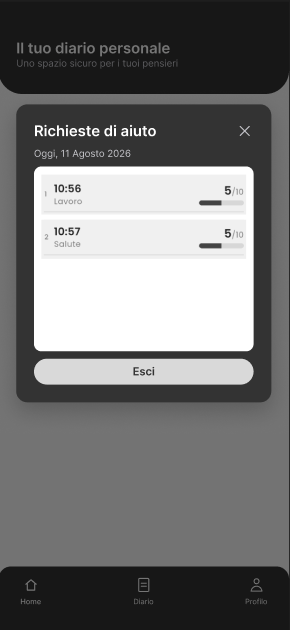
\includegraphics[height=8cm]{imgs/wireframes/popup-richieste-aiuto-final.png}
    \caption{Seconda versione del dettaglio delle richieste, raccolte in un riquadro unico}
    \label{fig:wireframe-richieste-b}
\end{figure}

\subsection{Spazio sicuro: la riflessione personale}
\label{subsec:wireframe-riflessione}

Per quanto riguarda la riflessione personale, la transizione in media fedeltà risulta pienamente soddisfacente.
Il riquadro si apre sopra il diario oscurato e destina quasi tutta la propria altezza all'area di scrittura, lasciandole attorno soltanto il titolo, il comando di chiusura e il pulsante di salvataggio.
L'assenza di elementi visivi aggiuntivi e l'isolamento del focus cognitivo evitano qualsiasi distrazione durante questo delicato momento di introspezione.
Rispetto allo sketch il comando conclusivo si riduce alla sola parola \enquote{Salva}, mentre il disegno a mano libera dichiarava insieme il salvataggio e l'uscita.

\begin{figure}[htbp]
    \centering
    
\includegraphics[height=8cm]{imgs/wireframes/popup-riflessione.png}
    \caption{Wireframe della riflessione personale}
    \label{fig:wireframe-riflessione}
\end{figure}

\section{Schermata Profilo: dati utente e preferenze di notifica}
\label{sec:wireframe-profilo}

La progettazione del profilo utente adotta un'architettura a card per raggruppare visivamente le informazioni e ridurre il carico cognitivo.
Il primo blocco è interamente dedicato ai dati personali (\textbf{REQ-11}), presentando campi di testo dal design pulito e un comando di salvataggio contestuale per evitare ambiguità operative.
La seconda sezione isola invece le impostazioni di sistema, affidando la gestione delle notifiche a un interruttore visivo dal feedback immediato e racchiudendo le opzioni di sicurezza secondarie in comandi ben distinti.

Particolare attenzione è stata riservata all'azione distruttiva di eliminazione dell'account.
Per prevenire tocchi accidentali, questo comando è stato fisicamente isolato dalle card principali e declinato con uno stile visivo privo di riempimento.
Questa strategia abbassa il peso gerarchico del pulsante, garantendo che la cancellazione avvenga solo tramite una volontà chiara e consapevole dell'utente.

\begin{figure}[htbp]
    \centering
    
\includegraphics[height=8cm]{imgs/wireframes/profilo.png}
    \caption{Wireframe del profilo}
    \label{fig:wireframe-profilo}
\end{figure}

\section{Direzione visiva: il mockup e la scelta della combinazione}
\label{sec:direzione-visiva}

I wireframe presentati fino a questo punto sono deliberatamente privi di colore, e questa assenza lascia aperta una domanda che nessuna schermata in scala di grigi può risolvere, ovvero quale aspetto debba avere un'applicazione destinata a essere aperta nei momenti peggiori della giornata.
Le linee guida viste a lezione indicano per questo passaggio l'uso di style tiles e mood board, cioè di proposte stilistiche alternative da confrontare fra loro, e raccomandano di non fermarsi alla prima idea, ma di costruirne più di una e di confrontarle a parità di contenuto.

Per condurre il confronto è stato generato un mockup interattivo in HTML che riproduce undici schermate dell'applicazione con la stessa struttura dei wireframe.
Il mockup espone quattro controlli, ovvero la palette dei colori, il carattere tipografico, lo stile chiaro o scuro delle card e, per le card scure, il grado di scurezza.
La scelta di un mockup navigabile anziché di semplici tavole di campioni risponde a un problema concreto, poiché una combinazione gradevole su un quadrato di colore può risultare inadeguata quando riveste un'intestazione, una barra di navigazione, un pulsante di emergenza e undici schermate diverse.
Cambiando un controllo tutte le schermate si aggiornano insieme, cosicché il confronto avvenga sempre a parità di contenuto.

L'esplorazione è partita da una prima veste a colori applicata alla schermata principale, che dà il nome alla palette Concept, e si è poi allargata ad altre tre direzioni costruite per allontanarsene ciascuna in un verso diverso.
Le quattro palette messe a confronto sono le seguenti.

\begin{table}[htbp]
    \centering
    \small
    \renewcommand{\arraystretch}{1.3}
    \begin{tabularx}{\textwidth}{L{1.9cm} L{3.4cm} L{3.1cm} X}
        \toprule
        \textbf{Palette} & \textbf{Intestazioni} & \textbf{Accento} & \textbf{Carattere della proposta} \\
        \midrule
        Concept & \texttt{\#174A46} teal profondo & \texttt{\#D8A5C5} rosa cipria & Naturale e calda, con un accento di tono attenuato \\
        Notturno & \texttt{\#1D2A4A} blu notte & \texttt{\#A79BD6} lavanda & Più fredda e istituzionale, vicina alle applicazioni di meditazione \\
        Terra & \texttt{\#3B4A3E} verde bosco & \texttt{\#DFA079} terracotta & Materica e avvolgente, con un accento caldo che tende all'arancione \\
        Bruma & \texttt{\#2A3840} ardesia & \texttt{\#93BFCB} azzurro polvere & Quieta e distaccata, con contrasti attenuati \\
        \bottomrule
    \end{tabularx}
    \caption{Le quattro palette messe a confronto nel mockup}
    \label{tab:palette}
\end{table}

\begin{figure}[htbp]
    \centering
    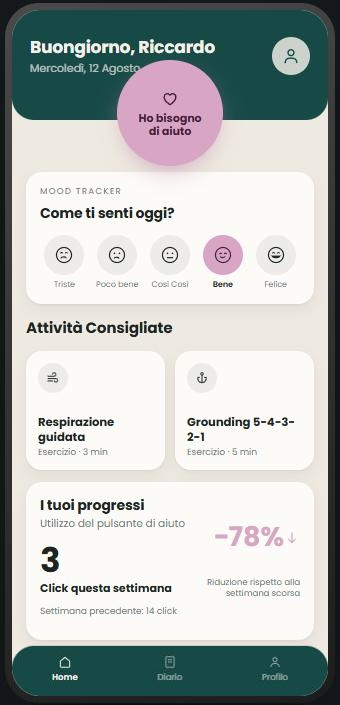
\includegraphics[height=7cm]{imgs/mockup/palette-concept.png}\hfill
    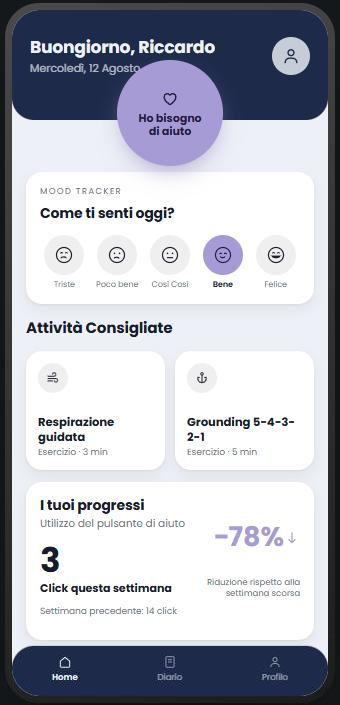
\includegraphics[height=7cm]{imgs/mockup/palette-notturno.png}\hfill
    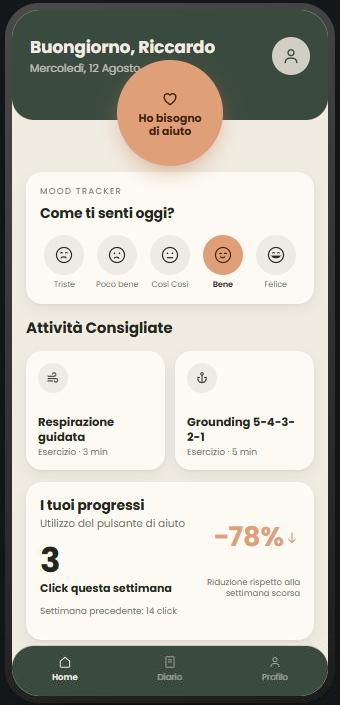
\includegraphics[height=7cm]{imgs/mockup/palette-terra.png}\hfill
    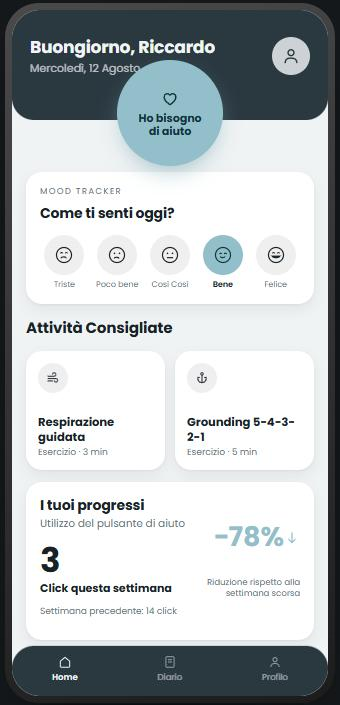
\includegraphics[height=7cm]{imgs/mockup/palette-bruma.png}
    \caption{La schermata principale nelle quattro palette messe a confronto: Concept, Notturno, Terra e Bruma}
    \label{fig:palette}
\end{figure}

La Figura \ref{fig:palette} riproduce la schermata principale nelle quattro varianti, nell'ordine della tabella, e mostra quanto una stessa struttura cambi di temperatura al variare della sola combinazione cromatica.

La combinazione adottata unisce la palette Concept, il carattere morbido dalle forme tondeggianti e le card chiare.
Il confronto fra le palette è stato condotto rispetto a tre criteri fissati prima di guardare le varianti, e ciascuno di essi ne ha esclusa una.
Il primo riguarda l'accento, che riveste il pulsante di richiesta di aiuto, e discende dall'analisi dei competitor: il rosso adottato da Rootd e da Dare induce urgenza anziché rassicurazione, e il colore dell'accento non deve quindi ricadere nella gamma dei segnali di avviso.
Il criterio esclude Terra, il cui terracotta tende all'arancione.
Il secondo riguarda la leggibilità sulle schermate intere, ed esclude Bruma, i cui contrasti attenuati indeboliscono proprio le scritte che devono restare leggibili quando l'utente sta male.
Il terzo riguarda il tono, ed esclude Notturno, più freddo e istituzionale, che avvicina Vivo alle applicazioni di meditazione da cui il progetto intende distinguersi.
Resta Concept, il cui rosa cipria non richiama né un allarme né una tinta fredda.
La scelta è ricaduta sulla proposta di partenza, ma solo dopo che le alternative erano state costruite e osservate sulle schermate intere, per verificare se una di esse reggesse meglio i tre criteri.

Il carattere morbido è stato scelto per coerenza con il tono dell'applicazione, poiché le forme tondeggianti risultano meno perentorie di quelle tecniche o editoriali.
Le card chiare, infine, sono state preferite a quelle scure ipotizzate nei wireframe perché mantengono le schermate leggibili anche con la luminosità del telefono abbassata, e con esse il quarto controllo del mockup, il grado di scurezza delle card, ha smesso di avere oggetto.
Card e fondo restano però due bianchi caldi vicini fra loro, e il solo colore non basta a distinguerli: le card sono quindi sollevate da un'ombra tinta con il teal della palette, che ne segna il confine senza bordi marcati e senza il grigiore che un'ombra nera produrrebbe sul fondo crema.
